\section{Warm Up: Feature Expansion}
\label{sec:feature-expansion}

[10 points total] Consider an instance space consisting of points on
the two dimensional plane $(x_1,x_2)$. Let $\mathcal{C}$ be a concept
class defined on this instance space. Each function
$f_r \in \mathcal{C}$ is defined by a radius $r$ as follows:
\[
f_r(x_1, x_2) = 
\begin{cases}
  +1  & \text{if } x_1^2 +x_2^2 - 2x_1 \leq r^2 \\
  -1 & \text{else}
\end{cases}
\]
This hypothesis class is definitely not separable in $\mathbb{R}^2$.
That is, there is no $w_1, w_2$ and $b$ such that $f_r(x_1, x_2) =
sign(w_1 x_1 + w_2 x_2 + b)$ for any $r$. 

\begin{enumerate}
\item ~[4 points] Construct a function $\phi(x_1,x_2)$ that maps
  examples to a new space, such that the positive and negative
  examples are linearly separable in that space? That is, after the
  transformation, there is some weight vector $\bw$ and a bias $b$
  such that $f_r(x_1, x_2) = sign(\bw^T\phi(x_1, x_2) + b)$ for any
  value of $r$.

  (Note: This new space need not be a two-dimensional space.)

  \begin{itemize}
    \item The distribution of the postive cases are in a circle that is centered around $(1,0)$. This can be mapped into 3-dimensions by using a Gaussian Distribution over the data. An alternative equation to the problem is $(x-1)^{2}+y^{2}\leq r^{2}+1$ which describes a cirlce of radius $\sqrt{r^{2}+1}$. Then, a plane at $Z=0.1$ (or some other small value for $Z$ to bisect the data) can be used to bisect the data. The formula that would be used is

\[
\phi(x_{1},x_{2}) = \exp\left(-\left(\frac{(x_{1}-1)^{2}}{2\sqrt{r^{2}+1}}\right) + \left(\frac{x_{2}^{2}}{2\sqrt{r^{2}+1}} \right)  \right)
\]

Which will create a Gaussian distribution in the z-dimension for positive examples and wouldn't change anything for the negative examples, which a hyperplane can bisect the two.
  \end{itemize}

\item ~[3 points] If we change the above function to: 
  \[
  g_r(x_1,x_2) = 
  \begin{cases}
    +1 & \text{if } x_1^2 -x_2^2 \leq r^2 \\
    -1 & \text{else}
  \end{cases}
  \]

  Does your $\phi(x_1,x_2)$ make the above linearly separable?  If so
  demonstrate how. If not prove that it does not.

\begin{itemize}
  \item It is trivially seen that $\phi(x_{1},x_{2})$ {\em cannot} make $g_{r}(x_{1},x_{2})$ linearlly separable as $\phi$ was a gaussian distribution in the shape of a cirlce. This allowed to raise the positive points above the axis. $g_{r}$ is a hyperbola, and therefore cannot be linarly separated by a gaussian distribution.
\end{itemize}

\item ~[3 points] Does $\phi(x_1,x_2) = [x_1,x_2^2]$ make the function
  $g_r$ above linearly separable? If so demonstrate how. If not prove
  that it does not.

\begin{itemize}
\item This can be shown graphically that this is {\em not} the case for all $r$. By taking the plots and plotting them in the $3^{rd}$ dimension, it can be trivially seen that there is no segment/hyper plane that can be drawn through the data. Figure~\ref{fig:3Dplot} shows the plot of $x^{2}-y^{2}\leq 2^{2}$, while Figure~\ref{fig:Contourplot} is of taking the data points in Figure~\ref{fig:3Dplot} and squaring the $y$ value, while keeping the classificataions.

%\item This can be shown graphically that it is the case. By taking the plots and plotting them in a higher $3^{rd}$ dimension, it can be trivally seen that there is a segment/hyper plane that can be drawn through the data. Figure~\ref{fig:3Dplot} shows the function plotted in 3 dimensions while Figure~\ref{fig:Contourplot} makes the bisection point easier to see by plotting it in two dimensions.

\begin{figure}
\centering
\begin{minipage}{.5\textwidth}
  \centering
  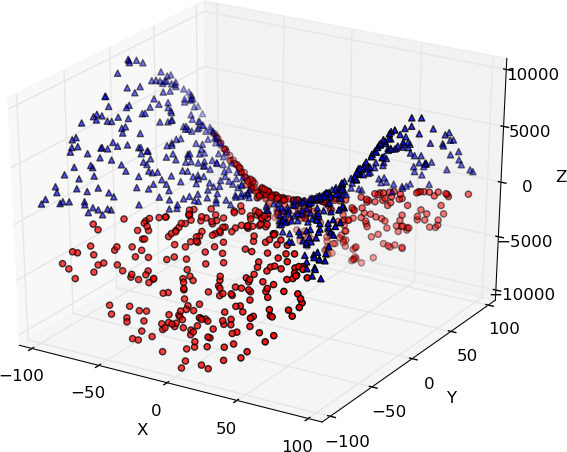
\includegraphics[width=\linewidth]{normal-1000-3.png}
  \captionof{figure}{Plot of $x^{2}-y^{2}\leq 2^{2}$}
  \label{fig:3Dplot}
\end{minipage}%
\begin{minipage}{.5\textwidth}
  \centering
  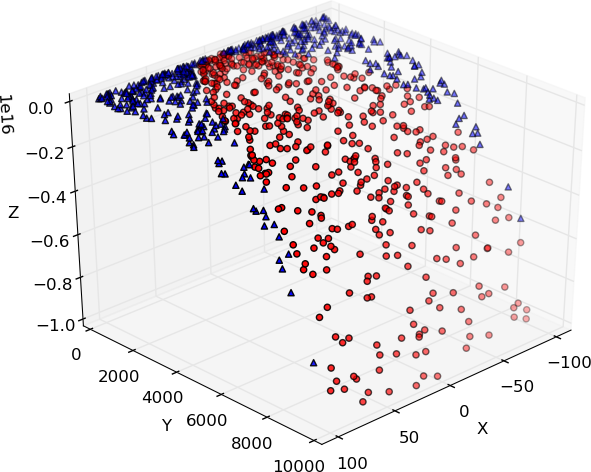
\includegraphics[width=\linewidth]{phi-1000-3.png}
  \captionof{figure}{Plot of $\phi(x,y)$}
  \label{fig:Contourplot}
\end{minipage}
\end{figure}
\end{itemize}

\end{enumerate}


%%% Local Variables:
%%% mode: latex
%%% TeX-master: "hw3"
%%% End:
